\documentclass{ctexart}
\usepackage{ctex}
\usepackage{graphicx}
\title{孙婷婷事件中的法律问题}
\begin{document}
\maketitle
\tableofcontents
\section{引言}
昨天下午,孙婷婷在她自己的微博上发布了长篇自白《我是孙婷婷,我要站出来》。 详细讲述了她无辜被拘留和在看守所遭遇的一系列非人待遇。她在自白的最后, 提出了十个问题,矛头直指广州番禺警方在这起案件中的做法。
\begin{figure}
  \centering
  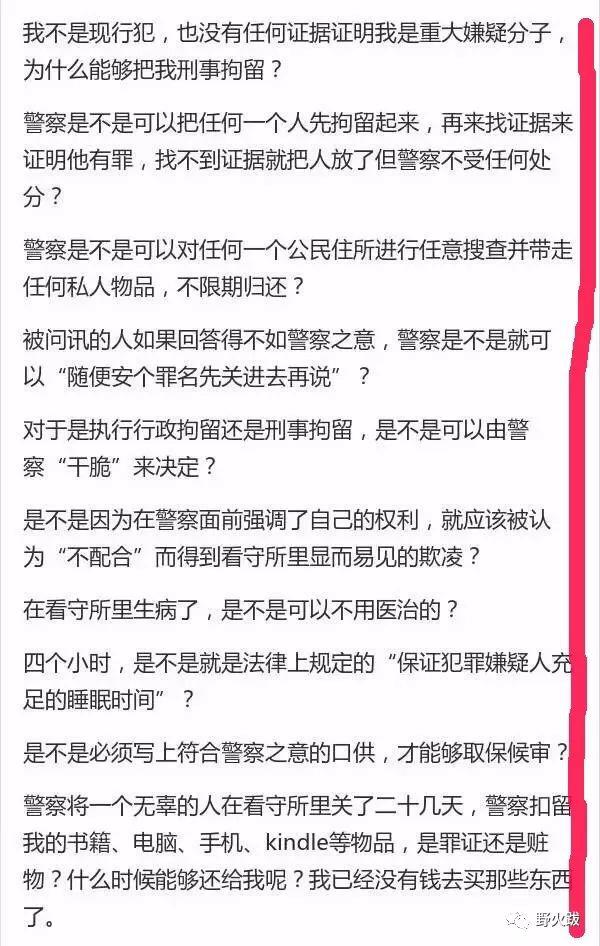
\includegraphics[width=300pt]{page1image.jpg}
  \caption{孙婷婷自白(部分)}
\end{figure}
下面我想就孙婷婷案所涉及的法律问题详细地分析下。 \par
如果孙婷婷所说的是真的,那么广州番禺警方在拘留、定罪、没收物品归还、看
守所虐待方面,很有可能面临严重违法!
\par
孙婷婷接下来可以要求该公安机关确认其刑事拘留违法,然后申请国家赔偿。
\section{问题}
\subsection{拘留违法问题}
\begin{quotation}
  “我不是现行犯,也没有任何证据证明我是重大嫌疑分子,为什么能够把我刑事 拘留?” “警察是不是可以把任何一个人先拘留起来,再来找证据来证明他有罪,找不到 证据就把人放了但警察不受任何处分?”
\end{quotation}\par
答:根据中国法律,刑事拘留是公安机关、人民检察院临时剥夺现行犯或者重大 嫌疑分子自由的强制方法。刑事拘留有一定条件,番禺警方不能随意拘留,也不 能先拘留后找证据。
\par
2012 年修正的《刑事诉讼法》第八十条规定了公安机关行使刑事拘留的条件:
\begin{quotation}
  第八十条 公安机关对于现行犯或者重大嫌疑分子,如果有下列情形之一的,可 以先行拘留:\par
(一)正在预备犯罪、实行犯罪或者在犯罪后即时被发觉的; \par(二)被害人或者在场亲眼看见的人指认他犯罪的;\par
(三)在身边或者住处发现有犯罪证据的;\par (四)犯罪后企图自杀、逃跑或者在逃的;\par (五)有毁灭、伪造证据或者串供可能的;\par (六)不讲真实姓名、住址,身份不明的;\par (七)有流窜作案、多次作案、结伙作案重大嫌疑的。
\end{quotation}\par
2013 年 1 月 1 日起生效的《公安机关办理刑事案件程序》第一百二十条同刑诉 第八十条。\par
解读一下法条,即公安机关进行刑事拘留必须同时具备两个条件:\par
其一,拘留的对象是现行犯或者是重大嫌疑分子。\par
现行犯是指正在实施犯罪的人,重大嫌疑分子是指有证据证明具有重大犯罪嫌疑 的人。
\par
其二,具有刑诉八十条列举的法定的七种紧急情形之一。\par
\medskip
我们来看当事人孙婷婷是否符合这两个条件;孙当然不是现行犯,警方最多也只 能牵强地将其认定为重大嫌疑分子(也需要初步证据和一定的嫌疑性);而法定 紧急情形中,只有“(三)在身边或者住处发现有犯罪证据”可能符合,前提是警方 确实搜查出了孙从事犯罪活动的罪证。
\medskip
而如果警方没有相应证据证明其是重大犯罪嫌疑人,且没有搜查出犯罪罪证,那 么番禺警方对公民孙婷婷的的刑事拘留行为可能涉嫌错误拘留或违法拘留。如果
这样的话,那么:\par
\medskip
首先,番禺警方应当承担国家赔偿责任并赔礼道歉\par
\begin{quotation}
国家赔偿法(2012 年修正)第十五条第一项规定:“对没有犯罪事实或者没有事 实证明有犯罪重大嫌疑的人错误拘留的”,受害人有取得赔偿的权利,即有权获 得侵犯人身自由赔偿金。\par

第十九条规定,行使国家侦查、检察、审判、监狱管理职权的机关及其工作人员 在行使职权时侵犯公民、法人和其他组织的合法权益造成损害的,该机关为赔偿 义务机关。\par
对没有犯罪事实或者没有事实证明有犯罪重大嫌疑的人错误拘留的,作出拘 留决定的机关为赔偿义务机关。\par
第三十条还规定,对于因错误刑事拘留,并造成受害人名誉权、荣誉权损害的, 侵权机关应当在侵权行为影响的范围内,为受害人消除影响,恢复名誉,赔礼道 歉。\par
\end{quotation}\par
其次,根据拘留时是否有主观故意(是判断错误还是明知故犯、栽赃陷害) 番 禺警方涉嫌错误拘留或违法拘留。\par
前者要接受内部纪律处分,后者则构成犯罪要接受刑事制裁。
\subsection{定罪问题}
\begin{quotation}
  “被问询的人如果回答得不如警察之意,警察是不是就可以”随便安个罪名先关进 去再说”
\end{quotation}\par
答:关进去当然不能是“随便安个罪名”关进去——刑事拘留是要有条件的。刑事 拘留的条件(回答 1)\par
\begin{quotation}
  公安机关办理刑事案件程序规定》\par 第三条:公安机关在刑事诉讼中的基本职权,是依照法律对刑事案件立案、侦查、 预审;决定、执行强制措施\par
  第一百八十七条:公安机关对已经立案的刑事案件,应当及时进行侦查,全面、 客观地收集、调取犯罪嫌疑人有罪或者无罪、罪轻或者罪重的证据材料。\par  第一百八十八条 :公安机关经过侦查,对有证据证明有犯罪事实的案件,应当 进行预审,对收集、调取的证据材料的真实性、合法性及证明力予以审查、核实。\par  第一百八十九条 :公安机关侦查犯罪,应当严格依照法律规定的条件和程序采 取强制措施和侦查措施,严禁在没有证据的情况下,仅凭怀疑就对犯罪嫌疑人采 取强制措施和侦查措施\par
\end{quotation}\par
对于执行行政拘留还是刑事拘留,是不是可以由警察”干脆”来认定?\par
答:刑事拘留和行政拘留两者差别巨大,存在着罪与非罪的界限。 刑事拘留适用于刑事案件中涉嫌犯罪的现行犯或者重大嫌疑分子。
行政拘留适用于有一般违法行为的人。 刑事拘留的行使应当满足法定的条件(回答 1)
\subsection{搜查问题}
\begin{quotation}
  “警察是不是可以对任何一个公民住所进行任意搜查并带走任何私人物品,不限 期归还?”
\end{quotation}\par
答:根据中国法律规定,警察当然不可以这样。
\begin{quotation}
  1.住宅权是我国宪法保护的公民基本人权(宪法第三十九条规定:中华人民共和 国公民的住宅不受侵犯。禁止非法搜查或者非法侵入公民的住宅。)非经法定程 序,警察不得搜查。\par
  《刑事诉讼法》第一百三十六条:进行搜查,必须向被搜查人出示搜查证。在执行逮捕、拘留的 时候,遇有紧急情况,不另用搜查证也可以进行搜查。\par
  《公安机关办理刑事案件规定》第二百零六条:进行搜查,必须向被搜查人出示《搜查证》,执行搜查的侦查人员 不得少于二人。第二百零六条 执行拘留,逮捕的时候,遇有下列紧急情况之一 的,不用《搜查证》也可以进行搜查:(一)可能随身携带凶器的;(二)可能隐 藏爆炸、剧毒等危险物品的;(三)可能隐匿、毁弃、转移犯罪证据的;(四)可 能隐匿其他犯罪嫌疑人的;(五)其他突然发生的紧急情况。
  《治安管理处罚法》第八十七条 公安机关对与违反治安管理行为有关的场所、 物品、人身可以进行检查。检查时,人民警察不得少于二人,并应当出示工作证 件和县级以上人民政府公安机关开具的检查证明文件(检查证)。对确有必要立 即进行检查的,人民警察经出示工作证件,可以当场检查,但检查公民住所应当 出示县级以上人民政府公安机关开具的检查证明文件。
\end{quotation}\par
总结一下法条,即番禺警方在搜查住宅时,必须向孙婷婷出示搜查证,除非搜查 时满足法定的紧急情况。而番禺警方既没有出示搜查证,而孙婷婷一介女子存在 “随身携带凶器”、“隐藏爆炸、剧毒等危险物品”等情况的可能性又极小,如无其 他证据证明其符合法定危急状态,那么番禺警方可能涉嫌程序违法。
\subsection{扣押物品归还问题}
\begin{quotation}
  “警察扣押我的书籍、电脑、手机、kindle 等物品,是罪证还是赃物,什么时候能
够还给我呢?”
\end{quotation}\par
答:根据中国法律规定,警方搜查时只能扣押与案件有关物品,其扣押物品应当
尽快查明是否有关,无关则三日内归还。
\begin{quotation}
 《刑事诉讼法》
第一百三十九条 在侦查活动中发现的可用以证明犯罪嫌疑人有罪或者无罪的各
种财物、文件,应当查封、扣押;与案件无关的财物、文件,不得查封、扣押。 对查封、扣押的财物、文件,要妥善保管或者封存,不得使用、调换或者损毁。 第一百四十三条 对查封、扣押的财物、文件、邮件、电报或者冻结的存款、汇 款、债券、股票、基金份额等财产,经查明确实与案件无关的,应当在三日以内 解除查封、扣押、冻结,予以退还。\par
2015 年公安部颁布的《公安机关涉案财物管理若干规定》
第六条 公安机关对涉案财物采取措施后,应当及时进行审查。经查明确实与案 件无关的,应当在三日以内予以解除、退还,并通知有关当事人。对与本案无关, 但有证据证明涉及其他部门管辖的违纪、违法、犯罪行为的财物,应当依照相关 法律规定,连同有关线索移送有管辖权的部门处理。
\end{quotation}\par
\subsection{看守所虐待问题}
是不是因为在警察面前强调了自己的权利,就应该被认为”不配合”而得到看守所
里显而易见的欺凌?\par
答:根据我国现行法律,这是违法行为。
\begin{quotation}
  第二百四十八条 【虐待被监管人罪】监狱、拘留所、看守所等监管机构的监管 人员对被监管人进行殴打或者体罚虐待,情节严重的,处三年以下有期徒刑或者 拘役;情节特别严重的,处三年以上十年以下有期徒刑。致人伤残、死亡的,依照 本法第二百三十四条、第二百三十二条的规定定罪从重处罚。”
\end{quotation}
在看守所里生病了,是不是可以不用医治的?
答:根据我国现行法律,这是违法行为。
\begin{quotation}
  国务院《中华人民共和国看守所条例 》
  第二十六条 看守所应当配备必要的医疗器械和常用药品。人犯患病,应当给予 及时治疗;需要到医院治疗的,当地医院应当负责治疗;病情严重的可以依法取 保候审。\par
  《中华人民共和国看守所条例实施办法》
第三十一条 对患病的人犯要及时治疗。人犯服药,看守干警要在场监视。发现 人犯患有传染病要立即隔离治疗。病情严重的,可以住院治疗;如办案机关决定 变更强制措施时,依照规定办理。
\end{quotation}
四个小时,是不是就是法律上规定的”保证犯罪嫌疑人充足的睡眠时间”?\par
答:根据我国现行法律法规,这是违法行为。
\begin{quotation}
  国务院《中华人民共和国看守所条例 》
第二十五条 人犯每日应当有必要的睡眠时间和一至两小时的室外活动。
\end{quotation}
是不是必须写上符合警察之意的口供,才能够取保候审?\par
答:根据我国现行法律法规,这是违法行为。
\begin{quotation}
  《刑事诉讼法》
第六十九条 被取保候审的犯罪嫌疑人、被告人应当遵守以下规定: \par(一)未经执行机关批准不得离开所居住的市、县;\par (二)在传讯的时候及时到案;\par
(三)不得以任何形式干扰证人作证;\par
(四)不得毁灭、伪造证据或者串供。\par 人民法院、人民检察院和公安机关可以根据案件情况,责令被取保候审的犯罪嫌 疑人、被告人遵守以下一项或者多项规定:
(一)不得进入特定的场所;\par (二)不得与特定的人员会见或者通信;\par (三)不得从事特定的活动;\par (四)将护照等出入境证件、驾驶证件交执行机关保存。
\end{quotation}
警方可以责令嫌疑人提交遵守相应规定的保证书,但是从来没有规定说“必须写 上符合警察之意的口供”
\subsection{其他问题}
\subsubsection{看守所可能涉嫌超期羁押}
对于公安机关依法决定和执行的刑事拘留,拘留的期限是法律分别规定的公安机 关提请人民检察院批准逮捕的时间和人民检察院审查批准逮捕的时间的总和。\par
公安机关对被拘留的人认为需要逮捕的,应当在拘留后的 3 日以内,提请人民检 察院审查批准。在特殊情况下,经县级以上公安机关负责人批准,提请审查批准 的时间可以延长 1 日至 4 日。对于流窜作案、多次作案、结伙作案的重大嫌疑分 子,经县级以上公安机关负责人批准,提请审查批准的时间可以延长至 30 日。 人民检察院应当自接到公安机关提请批准逮捕书后的 7 日以内,作出批准逮捕或 者不批准逮捕的决定。人民检察院不批准逮捕的,公安机关应当在接到通知后立 即释放犯罪嫌疑人,并且将执行情况及时通知人民检察院。对于需要继续侦查, 并且符合取保候审、监视居住条件的,依法取保候审或者监视居住。 \par 人民检察院对直接受理的案件中被拘留的人,认为需要逮捕的,应当在 14 日内 作出决定。在特殊情况下,决定逮捕的时间可以延长 1 日至 3 日。对于不需要逮 捕的,应当立即释放。对于需要继续侦查,并且符合取保候审监视居住条件的, 依法取保候审或者监视居住。 \par 综上所述,一般情况下,刑事诉讼拘留的期限最长为 14 日。流窜作案、多次作 案、结伙作案的重大嫌疑分子,拘留期限最长为 37 日。\par
根据公安部《规定》第 110 条规定,流窜作案,是指跨市、县范围连续作案,或 者在居住地作案后逃跑到外市、县继续作案;多次作案,是指 3 次以上作案;结伙 作案,是指 2 人以上共同作案。\par
本案中的孙婷婷,显然不符合“流窜作案、多次作案、结伙作案的重大嫌疑分子”
的条件。事实上,对她的拘押时间已经超过了法定最多的 14 天。
\subsubsection{救济途径}

先要求该公安机关确认其刑事拘留违法,然后可以申请国家赔偿。但如果该公安 机关拒不确认的话,则不能直接申请赔偿,只能通过向其上级公安机关等部门申 诉来谋求解决。\par
\begin{quotation}
  《国家赔偿法》\par
  第十七条 行使侦查、检察、审判职权的机关以及看守所、监狱管理机关及其工 作人员在行使职权时有下列侵犯人身权情形之一的,受害人有取得赔偿的权利: (一)违反刑事诉讼法的规定对公民采取拘留措施的,或者依照刑事诉讼法规定的 条件和程序对公民采取拘留措施,但是拘留时间超过刑事诉讼法规定的时限,其 后决定撤销案件、不起诉或者判决宣告无罪终止追究刑事责任的; \par(四)刑讯逼供或者以殴打、虐待等行为或者唆使、放纵他人以殴打、虐待等行为 造成公民身体伤害或者死亡的;\par
  第二十一条 行使侦查、检察、审判职权的机关以及看守所、监狱管理机关及其 工作人员在行使职权时侵犯公民、法人和其他组织的合法权益造成损害的,该机 关为赔偿义务机关。对公民采取拘留措施,依照本法的规定应当给予国家赔偿的,作出拘留决定的机 关为赔偿义务机关 \par
  第二十三条 赔偿义务机关应当自收到申请之日起两个月内,作出是否赔偿的决 定。\par
  第二十四条 赔偿义务机关在规定期限内未作出是否赔偿的决定,赔偿请求人可 以自期限届满之日起三十日内向赔偿义务机关的上一级机关申请复议。\par
  第二十五条 复议机关应当自收到申请之日起两个月内作出决定。\par
  赔偿请求人不服复议决定的,可以在收到复议决定之日起三十日内向复议机关所 在地的同级人民法院赔偿委员会申请作出赔偿决定;复议机关逾期不作决定的, 赔偿请求人可以自期限届满之日起三十日内向复议机关所在地的同级人民法院 赔偿委员会申请作出赔偿决定。
\end{quotation}

综上所述:假设孙婷婷的自述都是真的,那么番禺警方孙婷婷一案中在拘留、搜 查、看守所关押、个人物品归还方面严重违反了我国现行法律法规。需要承担相 应的责任。\par
孙婷婷接下来可以要求该公安机关确认其刑事拘留违法,然后申请国家赔偿。
\end{document}